\documentclass[12pt]{article}
\linespread{1.25}
\usepackage{times}

\usepackage{pgfplots}
\pgfplotsset{compat = newest}
\usetikzlibrary{positioning, arrows.meta}
\usepgfplotslibrary{fillbetween}
\usepackage{amsmath}

\begin{document}

\begin{center}
\hspace*{-3cm}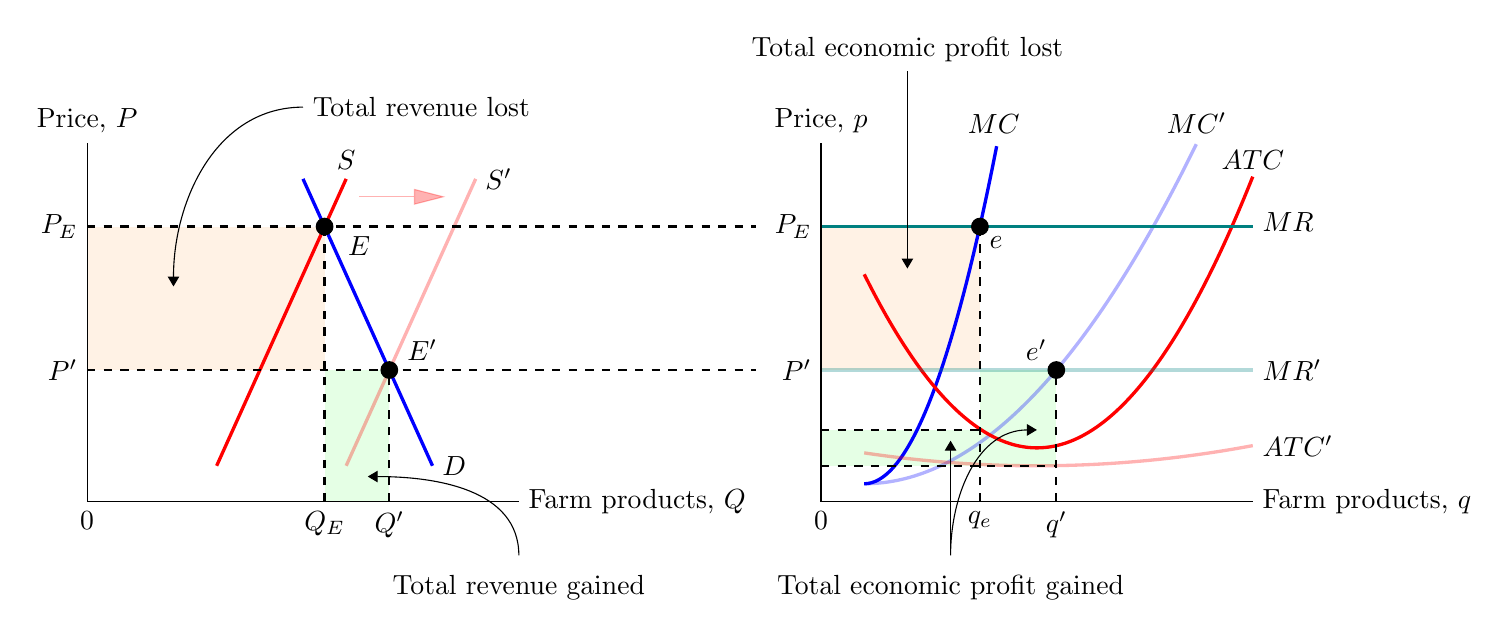
\begin{tikzpicture}
% Left-hand graph: Supply shift in market equilibrium
\begin{axis}[
scale = 0.8,
xmin = 0, xmax = 10,
ymin = 0, ymax = 10,
axis lines* = left,
xtick = {0}, ytick = \empty,
axis on top,
clip = false,
]
% Colouring areas
\fill[orange, opacity = 0.1] (0, 7.67) -- (0, 3.67) -- (5.5, 3.67) -- (5.5, 7.67);
\fill[green, opacity = 0.1] (5.5, 0) -- (5.5, 3.67) -- (7, 3.67) -- (7, 0);

% Supply and demand curves
\addplot[color = blue, very thick] coordinates {(5,9)(8,1)};
\addplot[color = red, very thick] coordinates{(3,1)(6,9)};
\addplot[color = red, opacity = 0.3, very thick] coordinates{(6,1)(9,9)};

% Dashed lines
\addplot[color = black, dashed, thick] coordinates {(0, 7.67)(15.5, 7.67)};
\addplot[color = black, dashed, thick] coordinates {(0, 3.67)(15.5, 3.67)};
\addplot[color = black, dashed, thick] coordinates {(5.5, 0)(5.5, 7.67)};
\addplot[color = black, dashed, thick] coordinates {(7, 0)(7, 3.67)};

% Coordinate points
\addplot[color = black, mark = *, only marks, mark size = 3pt] coordinates {(5.5, 7.67)(7, 3.67)};

% Labels
\node [right] at (current axis.right of origin) {Farm products, $Q$};
\node [above] at (current axis.above origin) {Price, $P$};
\node [below right=0pt and 5pt] at (5.5, 7.67) {$E$};
\node [above right = 0pt and 3pt] at (7, 3.67) {$E^\prime$};
\node [right] at (8, 1) {$D$};
\node [above] at (6, 9) {$S$};
\node [right] at (9, 9) {$S^\prime$};
\node [right, align=center] at (5, 11) {Total revenue lost};
\node [above, align=center] at (10, -3) {Total revenue gained};
\node [left] at (0, 7.67) {$P_E$};
\node [left] at (0, 3.67) {$P^\prime$};
\node [below] at (5.5, 0) {$Q_E$};
\node [below] at (7, 0) {$Q^\prime$};

% Arrows
\draw[-{Triangle[length=4mm, width=2mm]}, red, opacity = 0.3] (6.3, 8.5) to (8.3, 8.5);
\draw[-Triangle] (5, 11) to [out = 180, in = 90] (2, 6);
\draw[-Triangle] (10, -1.5)  to [out = 90, in = 0] (6.5, 0.7);
\end{axis}

% Right-hand graph: Price-taking firm
\begin{axis}[
scale = 0.8,
xmin = 0, xmax = 10,
ymin = 0, ymax = 10,
axis lines* = left,
xtick = {0}, ytick = \empty,
axis on top,
clip = false,
shift = {(axis cs: 17, 0)},
]
% Colouring areas
\fill[orange, opacity = 0.1] (0, 3.67) --  (3.68, 3.67)  -- (3.68, 7.67) -- (0, 7.67);
\fill[green, opacity = 0.1] (3.68, 1) -- (5.45, 1) -- (5.45, 3.67) -- (3.68, 3.67);
\fill[green, opacity = 0.1] (0, 1) -- (0, 2) -- (3.68, 2) -- (3.68, 1);

% Curves
\addplot [domain =1:10, restrict y to domain = 0:10, samples = 400, color = blue, very thick]{(x-1)^2+0.5};
\addplot [domain =1:10, restrict y to domain = 0:10, samples = 400, color = blue, opacity = 0.3, very thick]{(0.4*(x-1))^2+0.5};
\addplot [domain = 1:10, restrict y to domain = 0:10, samples = 400, color = red, very thick]{(0.55*(x-5))^2+1.5};
\addplot [domain = 1:10, restrict y to domain = 0:10, samples = 400, color = red, opacity = 0.3, very thick]{(0.15*(x-5))^2+1};
\addplot [domain = 0:10, restrict y to domain = 0:10, samples = 400, color = teal, very thick]{7.67};
\addplot [domain = 0:10, restrict y to domain = 0:10, samples = 400, color = teal, opacity = 0.3, very thick]{3.67};

% Dashed lines
\addplot[color = black, dashed, thick] coordinates {(3.68, 0)(3.68, 7.67)};
\addplot[color = black, dashed, thick] coordinates {(5.45, 0)(5.45, 3.67)};
\addplot[color = black, dashed, thick] coordinates {(0, 1)(5.45, 1)};
\addplot[color = black, dashed, thick] coordinates {(0, 2)(3.68, 2)};

% Coordinate points
\addplot[color = black, mark = *, only marks, mark size = 3pt] coordinates {(3.68, 7.67)(5.45, 3.67)};

% Labels
\node [right] at (current axis.right of origin) {Farm products, $q$};
\node [above] at (current axis.above origin) {Price, $p$};
\node [below right] at (3.68, 7.67) {$e$};
\node [above left] at (5.45, 3.67) {$e^\prime$};
\node [above] at (4, 10) {$MC$};
\node [above] at (10, 9) {$ATC$};
\node [right] at (10, 7.8) {$MR$};
\node [above] at (8.7, 10) {$MC^\prime$};
\node [right] at (10, 1.56) {$ATC^\prime$};
\node [right] at (10, 3.67) {$MR^\prime$};
\node [above] at (2, 12) {Total economic profit lost};
\node [above] at (3, -3) {Total economic profit gained};
\node [left] at (0, 7.67) {$P_E$};
\node [left] at (0, 3.67) {$P^\prime$};
\node [below] at (3.68, 0) {$q_e$};
\node [below] at (5.45, 0) {$q^\prime$};

% Arrows
\draw[-Triangle] (3, -1.5) to [in = 180, out = 90] (5, 2);
\draw[-Triangle] (3, -1.5) to (3, 1.7);
\draw[-Triangle] (2, 12) to (2, 6.5);
\end{axis}
\end{tikzpicture}\hspace*{-3cm}
\end{center}
\textbf{Figure 5-7:} The effect of a bumper harvest on the farm product market (L) and individual farmers (R). 

\end{document}